%  $Description: Author guidelines and sample document in LaTeX 2.09$
%
%  $Author: ienne $
%  $Date: 1995/09/15 15:20:59 $
%  $Revision: 1.4 $
%
%\documentclass[times, 10pt,twocolumn]{article}
%\documentclass[conference,final]{IEEEtran}
\documentclass[10pt,conference]{IEEEtran}
\usepackage{latex8}
\usepackage{times}

% Users' option
\usepackage{amssymb}
\usepackage{amsmath}
\usepackage{graphicx}
\usepackage{epstopdf}
\usepackage{color}
\topmargin=0.01in
\usepackage{multirow}
\usepackage{booktabs}
\newif\ifdraft
\drafttrue

\renewcommand{\multirowsetup}{\centering}
\renewcommand{\arraystretch}{1.2}
\def\nyc{\centering}

\ifdraft
\newcommand{\fixme}[1]{ { \bf{ ***FIXME: #1 }} }
\newcommand{\jhanote}[1]{ {\textcolor{red} { ***Jha: #1 }}}
\newcommand{\Nkimnote}[1]{ {\textcolor{green} { ***Nkim: #1 }}}
\newcommand{\skonote}[1]{ {\textcolor{blue} { ***Jeff: #1 }}}
\else
\newcommand{\jhanote}[1]{}
\newcommand{\Nkimnote}[1]{}
\newcommand{\fixme}[1]{}
\newcommand{\skonote}[1]{}
\fi
% End of users' option

%\documentstyle[times,art10,twocolumn,latex8]{article}

%-------------------------------------------------------------------------
% take the % away on next line to produce the final camera-ready version
\pagestyle{empty}

\newcommand{\up}{\vspace*{-1em}}
\newcommand{\upp}{\vspace*{-0.5em}}
\newcommand{\ts}{$T_{s}$}


%-------------------------------------------------------------------------
\title{A Framework for Coupled Multi-physics Simulations \skonote{some charming title?? emphasizing ''it can cover various kinds of applications in different requirement, main components can be replaced by other similar softwares, etc.''} }

\author{
 ~\\[-2em]
 Soon-Heum Ko$^{1,2}$, Nayong Kim$^{2}$, Shantenu Jha$^{3,2}$\\
 \small{\emph{$^{1}$National Supercomputing Centre, Lin\"{o}ping University, Lin\"{o}ping, Sweden}}\\
 \small{\emph{$^{2}$Center for Computation \& Technology, Louisiana State University, USA}}\\
 \small{\emph{$^{3}$Dept. of Elec. and Comp. Eng., Rutgers University, Piscataway, New Jersey, USA}}\\
% \small{\emph{$^{*}$Contact Author}}\\
}

%\thispagestyle{empty}

\begin{document}

\maketitle

\begin{abstract}
\skonote{It is written considering that we will develop the hybrid simulation framework where multiple distinct application codes are coupled. We shall decide first \textbf{whether we will focus only on a framework for a computationally coupled multiple executions in parallel or we will also cover the workflow between computational and experimental tasks scheduled in tandem.}}
we design and develop a multi-physics framework for coupled simulations 
in which scientific components (codes) are logically separated. 
Designed framework provides the interface between scientific 
components, the compiling service for different system architectures, a 
runtime environment for scheduling of coupled tasks, and data 
management/code versioning support. The framework is built by 
developing the data exchange interface between coupled codes, providing 
the compilation templates for specific architectures, adopting a BigJob 
abstraction, and using the PetaShare service. We apply this framework 
into the hybrid computational fluid dynamics - particle dynamics 
application to demonstrate its capability.
\end{abstract}
\up\up

%-------------------------------------------------------------------------
\section{Introduction and Motivation}

''Coupled scientific simulations'' will refer to the scientific 
research procedure which involves the data exchange between different 
components operating either in parallel or in tandem. In both cases, 
whether scientific tools are synchronously exchanging the information 
during a single run or individual tools iteratively give the feedback 
to their counterparts, scheduling the overall procedure and providing 
the data stream under the distributed computing infrastructure is a 
headache to domain scientists. It motivates the development of a 
framework for coupled multi-component applications, which provides the 
following capabilities:
%{\it Framework} is defined as ''an abstraction in which software providing generic functionality can be selectively changed by user code, thus providing application specific software.''~\cite{Framework} According to this definition, a coupled multi-component framework shall provide the following functionalities: 
(1) the framework provides the data interface between distinct tools,
(2) embedded softwares should be adaptive to different users' 
implementations, and 
(3) they should be removable/replaceable by users' preferences.

Two different strategies can be applied to designing a coupled multi-
component framework. One is to modularize all components and bind them 
into a single executable, and the other is to keep multiple standalone 
softwares and provide the interface between individual executable. The 
former is good for scheduling on most batch queue systems and 
effectively using allocated resources, while some restrictions on data 
structure or standard grammar may apply on users' codes. Also, the 
binary can be heavier since the executable might contain unused or non-
optimized functions for solving specific target applications. The other 
gives much freedom in writing the individual component but can cause a 
computational headache in scheduling these components in remote 
production systems. We consider that the integration to a single binary 
is recommendable if all software packages are tightly coupled together 
for a single task or they share most memory allocations. It is 
preferred to couple multiple components through the communication 
interface and the scheduling function if those packages are 
sequentially loaded or they have different code structures.
%This way is desirable if one simulation package is apparently lighter than the other or multiples of components are working together for a single application target, or all elements share a very similar data structure with variables or all elements can be scheduled in a sequential/tandem order on the simulation process. Cactus framework is one such example.

A runtime environment for a coupled multi-physics application 
\cite{CCGrid_Hybrid} has been developed previously. In this work, two 
coupled yet logically distributed scientific softwares have been 
effectively scheduled under the single batch queue allocation, by 
incorporating the load balancing capability on a BigJob abstraction 
\cite{repex_ptrsa}. It demonstrated that a Pilot-job formulation can 
ease the scheduling of a coupled application whose components are 
hardly packed into a single binary. However this runtime environment 
lacks the reusability because it only provides the scheduling 
functionality between already-coupled distinct application codes.

In this work, we design and develop a coupled multi-component 
framework. Along with the runtime environment between logically 
separated components, we also provide the standard interface between 
these coupled components and take care of the data 
management/versioning. The structure of a coupled simulation framework 
is introduced in Sec.~\ref{sec:design}. Specific softwares implemented in this framework are described in Sec.~\ref{sec:implementation}. A 
coupled multi-physics application and an experiment-computation 
integrated research procedure are presented in Sec.~\ref{sec:experiment}. 
Recommendation for future work and conclusions are presented in Sec. 
\ref{sec:futureworks} and Sec.~\ref{sec:conclusion}.



% -------------------------------------------------------------------------
\section{Design of a Coupled Simulation Framework}
\label{sec:design}

\subsection{Requirements}
\skonote{In this section, we shall contain \textbf{what functionality the framework should provide} in easy words.}

Packaging multiple components into a single binary is very tough if (1) 
each component uses very different computational kernels or (2) a 
manual processing/decision-making is included in one of solution 
procedures. A hybrid computational fluid dynamics (CFD) - molecular 
dynamics (MD) simulation is an example whose data structures are 
completely different so that it is fairly hard to incorporate 
application modules into a single binary. Another situation is 
occasionally observed when there is an iterative feedback between a 
numerical simulation and the experimental measurement. Most probably, 
the physical experiment involves the human labor of changing 
specimen/mockup after the numerical investigation, which cannot be 
digitalized. Figure~\ref{Fig:Overall_Flow} describes the solution 
procedure for these two multi-component simulations.


%%%%% FIGURE %%%%%
\begin{figure}[ht]
\centering
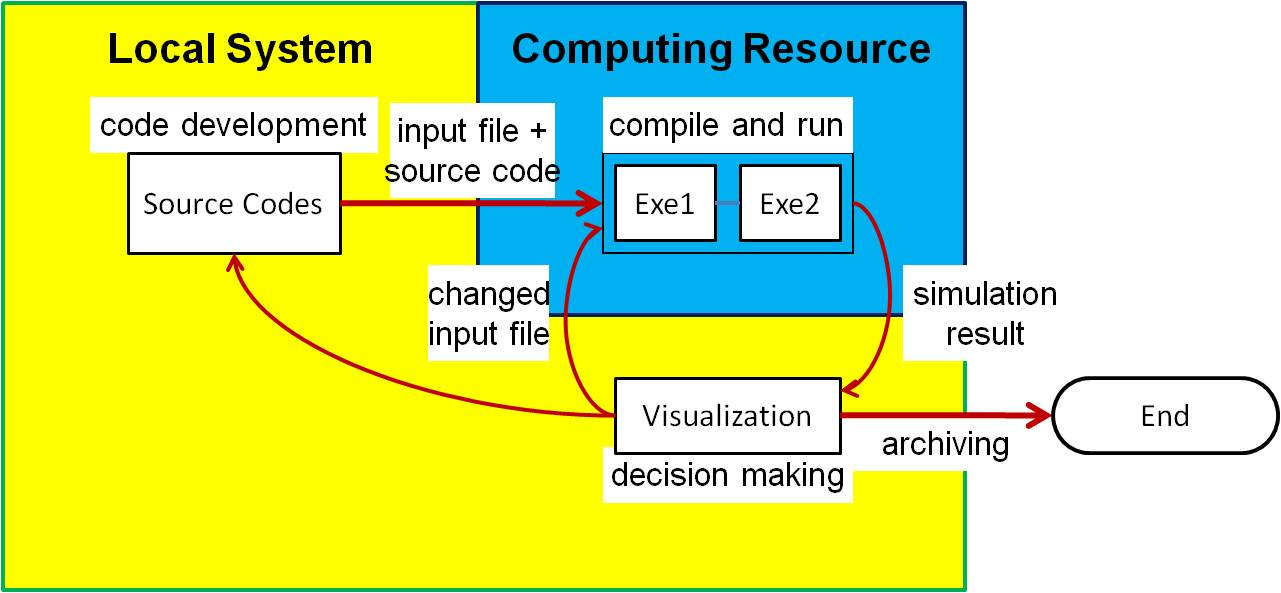
\includegraphics[width=0.8\linewidth]{Flow_Multiphysics_Simulation.jpg}
\vskip 0.2cm
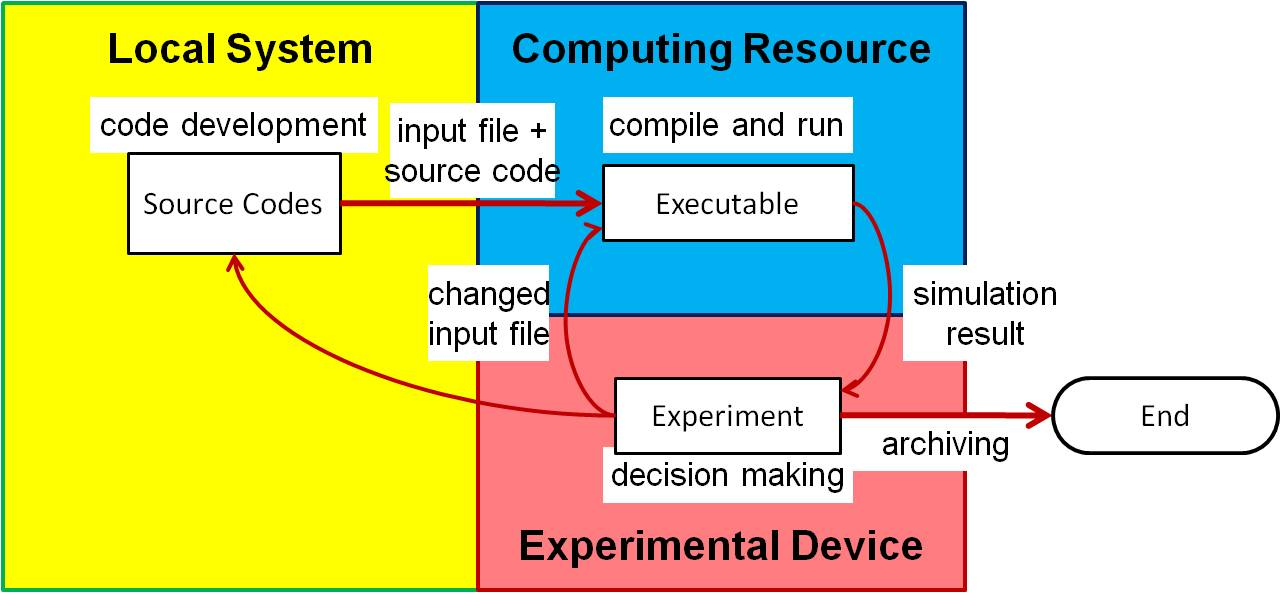
\includegraphics[width=0.8\linewidth]{Flow_Exp_and_Comp.jpg}
\vskip-0.2cm
\caption{\small 
{\bf Solution procedure of (1) coupled multi-physics simulations and 
(2) successive feedback between computations and experiments.} 
In both cases, frequent data transfer takes place between local and 
remote systems and a manual decision-making intervenes (either by 
visualizing the numerical solution or by performing the experimental 
measurement). In addition, the synchronous communication takes place
between co-scheduled computational components in case scietific 
softwares are coupled in parallel.}
\label{Fig:Overall_Flow}
\end{figure}
%%%%% FIGURE %%%%%


A coupled multi-component simulation framework should be capable of 
scheduling the overall procedure (workflow) and providing co-scheduled 
execution between multiple tasks (runtime environment). The workflow 
shall run middleware and scientific software packages according to the 
pre-described schedule. A runtime environment executes coupled multiple 
softwares in parallel, in the form of a virtually single executable 
under the batch queue system.

The functionality to handle the data flow (data management/archiving) and the standardised communicator for the coupled simulation (coupling interface) will provide more convenience in performing the coupled simulation and building coupled software packages. The framework should be capable of transerring data between distributed tools when each operation completes; Executables on remote computing facilities should be up-to-date when there is a change on the source code in the local server; Final solutions from multiple different parameter sets should be archived effectively. In addition, the capability of exchanging datasets between destinct softwares without the explicit and direct access between individual source code will ease the development of coupled scientific softwares. (or: the supprot of a standardised communicator between distinct codes will ease the development of coupled scientific softwares.)


\subsection{Design}
\skonote{In this section, we address \textbf{what functionality each group/service will provide and how we can give these services} in more professional terms.}

We design the concrete structure of a coupled multi-component simulation framework as presented in Fig.~\ref{Fig:Multicomponent_Framework}. Looking at the operation flow, the updated source code from the local machine replaces the old version in the remote computing resource and the individual source code is coupled together during the compilation, by the help of the external coupling interface. A runtime environment runs these distinct-yet-coupled executables concurrently. The solution is referenced by a scientist and the decision is made to accept/decline the numerical solution (either through the visualization or the experimental measurement). The acceptable solution is archived in the local server, or the new computation is performed by changing simulation parameters or source codes. In case the computation and the experimential measurement are coupled in sequence, compilation and job submission processes become simpler.


%%%%% FIGURE %%%%%
\begin{figure}[ht]
\centering
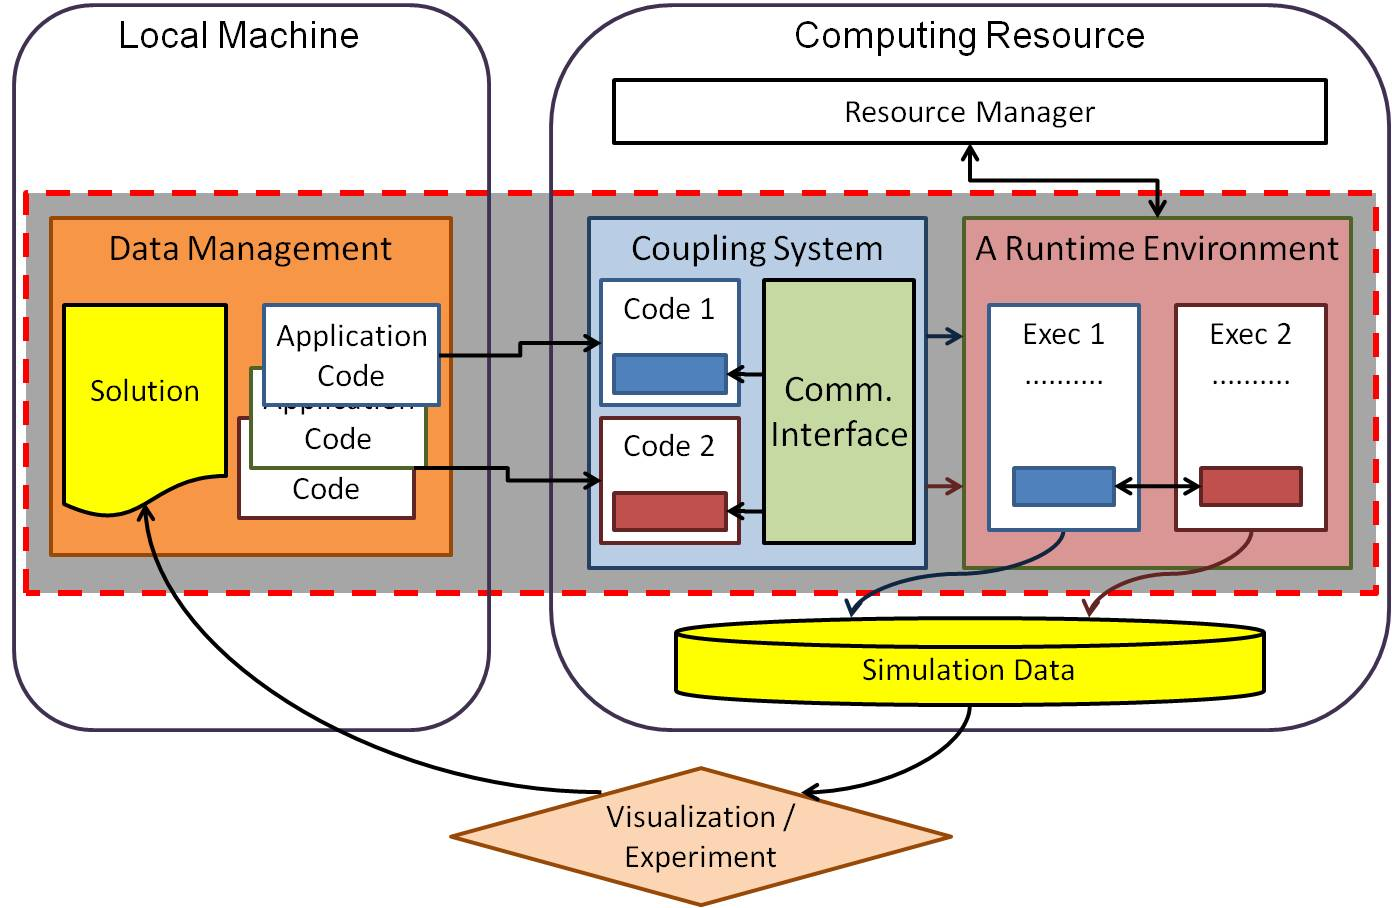
\includegraphics[width=0.8\linewidth]{Coupled_Framework_Diagram.jpg}
\vskip-0.2cm
\caption{\small {\bf Structure of a coupled multi-component application 
framework.} The framework is composed of three main packages: 
a data archiving/versioning service, a coupler and a runtime environment. 
A workflow script is running these packages according to the 
coupled simulation procedure.}
\label{Fig:Multicomponent_Framework}
\end{figure}
%%%%% FIGURE %%%%%


Data management service provides the data sharing among distributed computing facilities, updating the source codes on local and remote machines, and archiving final solutions. These functions can be implemented by running a couple of secure FTP commands; Installing a versioning service such as CVS (Concurrent Versioning System:~\cite{CVS}), SVN (Apache Subversion:~\cite{SVN}), or GIT (The fast version control system:~\cite{GIT}) on a central repository server is another way; Using a data Grid service such as PetaShare~\cite{PetaShare} can be helpful if sharing large-scale data on a distributed environment is of particular interest.

Coupling system provides the interface for the information exchange between distinct application codes and helps the compiling procedure in different system architectures. The coupling interface can be supported either in the form of a library which opens a file-based channel between distributed executables, or as a separate binary which binds all MPI communicators under a single MPI runtime environment. In either case, the interface function calls should be deployed in coupled source codes. Compilation system takes care of compiling individual scientific codes and coupling interface. It wraps up compiling options on users' makefiles to add the linkage with the coupling library and to apply optimal options for specific system architectures. A single wrap-up script along with templates which store optimal compilation options for known system architectures can provide these capabilities up to some extent; Some advanced compilation systems such as the Simulation Factory~\cite{SimFactory} can provide more functionality independent of different system architectures and configurations.

A runtime environment is designed to co-schedule and load-balance between coupled distinct tasks. The above issue is easily resolved by allocating a pilot-job in which coupled subtasks are effectively scheduled. A number of pilot-job implementations such as a Condor Glidein Job~\cite{Condor}, a BigJob abstraction~\cite{repex_ptrsa}, or a Pilot Factory~\cite{PilotFactory}, are present. Also, some supercomputing centers provide the capability of concurrently starting multiple jobs in the basic level.

% -------------------------------------------------------------------------
\section{Implementation}
\label{sec:implementation}
\skonote{In this section, we shall explain \textbf{how each service is implemented in our specific framework}.}

\subsection{Data Management and Archiving}

\subsection{Coupling System}
Coupling system services (1) the information exchange interface between coupled distinct codes, and (2) the Makefile-wrapper for specific system architectures. The former helps in writing the application code in a generic form and the latter enables compiling the program independent of the system architecture.

The coupling interface is provided in the form of a library. It acts to exchange registered variables between two codes. A ''separate'' library is linked to individual executable and the information exchange takes place between the library interfaces through the file-based communicator. Initially, parameters from users' codes, i.e., the communicator ID (any strings which define a set of coupled application) and the element ID (either 1 or 2), are registered to the library. Upon the calling of a \textit{send} function, the library stores passed data to the file communicator whose unique name is provided by the communicator ID and the element ID. In time of loading the \textit{recv} function, the library scans (and waits for) the data file from the counterpart and returns this dataset to the scientific code. Compared with the MPI-based communicator, the file I/O has the low latency/bandwidth and can have the stability issue in cases the resource experiences the unstability in file system. On the other hand, the file communicator library form does not require the dedicated resources compared with the separate MPI-based coupler and it is basically free to cooperate on distributed resources.

The Makefile-wrapper overwrites the user's Makefile so as to link the coupling interface and to apply optimal compiling options. It consists of a wrapper script and a number of templates which specify optimal compiling options for well-known system architectures. The script replaces user's compiling flag with the recommended ones for that system architecture and adds the linking flag of the coupling interface. The wrapper gets the location and the name of user's Makefile, as well as the location of a coupling library. By default, they are set to be \textit{./}, \textit{Makefile}, and \textit{../Lib}. The wrapper also accepts user's flags from the input file, which prioritize over the recommended configuration for that system architecture.


\subsection{Runtime Environment}
A BigJob is a pilot-job implementation under the simple API for grid applications (SAGA)~\cite{saga_url}. SAGA provides a simple, POSIX-style API to the most common grid functions at a sufficiently high-level of abstraction in order to be independent of diverse and dynamic grid environments. The SAGA specification defines interfaces for the most common grid-programming functions grouped as a set of functional packages. Thanks to various adaptors in SAGA, the BigJob application is infrastructure-neutral, which is the strength over other
Pilot-job implementations.

We apply the previously-established BigJob runtime environment for coupled multi-physics applications~\cite{CCGrid_Hybrid}. The load balancing function is turned off since it requires relevant changes (time checking function and checkpointing capability) in the application code. We directly submit a job to the remote batch queue system in case the sequential feedback process between a computation and an experiment is of interest.


\subsection{Workflow Engine}
The workflow engine consists of a number of hierarchical scripts. The main script \textit{hybrid} loads each relevant module according to the procedure of coupled simulations. 
(introduce each service, along with how it operates. Especially, about the first procedure which copies local files to petashare location)
shall provide the hierarchical structure where modules will run.


The first characteristic is the simplicity. (minimize variables to edit, while yours can still handle many parameters if not set default.)


The second and more important feature is the controllability. (you can start from the middle, skip some procedures, restart from where it ended.)



% -------------------------------------------------------------------------
\section{Numerical Experiments}
\label{sec:experiment}

% -------------------------------------------------------------------------
\section{Further Achievements}
\label{sec:futureworks}

%-------------------------------------------------------------------------
\section{Conclusions}
\label{sec:conclusion}

%-------------------------------------------------------------------------
\section*{Acknowledgment}

%-------------------------------------------------------------------------
%\nocite{ex1,ex2}
\bibliographystyle{latex8}
%\bibliographystyle{IEEEtran}
\bibliography{Bibs/Hybrid,Bibs/saga,Bibs/saga-related}


\end{document}


